\section{Auswertung} 

\subsection{Untersuchung der Störstellen in einem Acrylblock mit einem A-Scan}

\begin{flushleft}
    Für den ersten Teil des Versuches wurden die folgenden Abmessungen des Acrylblocks mit einer Schieblehre bestimmt.
\end{flushleft}

\begin{table}[H]
    \centering
    \caption{Entfernung der Löcher zur den Kanten.} 
    \label{Tabelle2}
    \begin{tabular} {c  c  c  c}
        \toprule
        {$ \text{Loch} $} &
        {$ \text{obere Kante} \mathbin{/} \unit{\milli\meter} $} &
        {$ \text{untere Kante} \mathbin{/} \unit{\milli\meter} $} &
        {$ \text{Durchmesser} \mathbin{/} \unit{\milli\meter} $} \\
        \midrule
        4  & 53,24  & 22    & 4,18 \\
        5  & 46,06  & 30    & 3,18 \\
        6  & 38,18  & 38,12 & 2,18 \\
        7  & 30,16  & 46,14 & 2,18 \\
        8  & 22,152 & 54,16 & 2,18 \\
        9  & 14,18  & 63    & 2,18 \\
        10 & 6,89   & 71    & 2,16 \\
        \bottomrule
    \end{tabular} 
\end{table}

\begin{align}
    \intertext{Für die Messung wurden sieben Löcher ausgewählt, in diesem Fall von Lochnummer vier bis zehn.
    Dabei werden die Werte aus Tabelle \ref{Tabelle1} als Literaturwerte angenommen.
    Die Lage, sowie die Größe aller Bohrungen, werden mit dem Impuls-Echo-Verfahren bestimmt.
    Der Acrylblock wird auf ein weiches Papiertuch platziert und mit einer $2\,\unit{\mega\hertz}$ Sonde von oben des Blockes gekoppelt.
    Das Koppelmittel ist Wasser.
    Mit Hilfe des A-Scans werden die verschiedenen Stellen auf Störstellen untersucht, die aus den Zeiten der Tiefe folgen.
    Bei bekannter Schallgeschwindigkeit, in diesem Fall $\text{c}_{\text{Acryl}} = 2730\, \frac{\unit{\meter}}{\unit{\second}}$ aus dem Literaturwert \cite{a2}, kann aus der Laufzeit t die Lage der Fehlstelle mit der Formel aus \ref{6} bestimmt werden.
    Die Anordnung wird nach der ersten Messung für die sieben Löcher umgedreht und erneut gemessen.
    Der Durchmesser der Löcher entspricht der Formel.}
    \text{d} = \text{h} - \text{s}_{\text{oben}} - \text{s}_{\text{unten}}. \label{9} 
    \intertext{Die Höhe des Acrylblockes wurde gemessen}
    \text{h} = 0,08005\,\unit{\meter}. \notag
    \intertext{Die Messungen werden in der Tabelle \ref{Tabelle3} notiert.} \notag
\end{align}

\begin{table}[H]
    \centering
    \caption{Messungen des ersten Arbeitsauftrages.} 
    \label{Tabelle3}
    \begin{tabular} {c  c  c  c  c  c}
        \toprule
        {$ \text{Loch} $} &
        {$ \text{t}_{\text{oben}} \mathbin{/} \unit{\micro\second} $} &
        {$ \text{s}_{\text{oben}} \mathbin{/} \unit{\milli\meter} $} &
        {$ \text{t}_{\text{unten}} \mathbin{/} \unit{\micro\second} $} &
        {$ \text{s}_{\text{unten}} \mathbin{/} \unit{\milli\meter} $} &
        {$ \text{d} \mathbin{/} \unit{\milli\meter} $} \\
        \midrule
        4  & 40,0 & $ 54,60 \pm 0,16 $ & 17,0 & $ 23,20 \pm 0,06 $ & $ 2,25 \pm 0,13 $ \\
        5  & 34,6 & $ 47,22 \pm 0,12 $ & 22,8 & $ 31,12 \pm 0,07 $ & $ 1,71 \pm 0,18 $ \\
        6  & 29,2 & $ 39,85 \pm 0,09 $ & 29,0 & $ 39,58 \pm 0,09 $ & $ 0,62 \pm 0,11 $ \\
        7  & 23,4 & $ 31,94 \pm 0,07 $ & 34,9 & $ 47,63 \pm 0,13 $ & $ 0,48 \pm 0,14 $ \\
        8  & 17,7 & $ 24,16 \pm 0,06 $ & 40,7 & $ 55,55 \pm 0,16 $ & $ 0,34 \pm 0,18 $ \\
        9  & 11,9 & $ 16,24 \pm 0,05 $ & 46,6 & $ 63,60 \pm 0,19 $ & $ 0,21 \pm 0,09 $ \\
        10 & 10,2 & $ 13,92 \pm 0,05 $ &   /  &         /          &         /         \\
        \bottomrule
    \end{tabular} 
\end{table}

\subsection{Bestimmung der Schallgeschwindigkeit}

\begin{flushleft}
    Zur Bestimmung der Schallgeschwindigkeit werden die jeweiligen Laufzeiten zu den Störstellen bestimmt.
    Da beim Impuls-Echo-Effekt die doppelte Strecke durchlaufen wird, werden die Laufzeiten halbiert.
    Die Länge der einzelnen Löcher wird aus der Tabelle \ref{Tabelle3} entnommen, sowie die dazugehörige Laufzeit aus \cite{a2}.
    Die Steigung der Gerade wird auf Hilfe einer linearen Regression ermittelt.
\end{flushleft}

\begin{align*}
    \intertext{Die lineare Regression liefert}
    c = (2961,74 \pm 121,36)\,\frac{\unit{\meter}}{\unit{\second}}\,.
\end{align*}

\begin{figure}[H] 
    \centering
    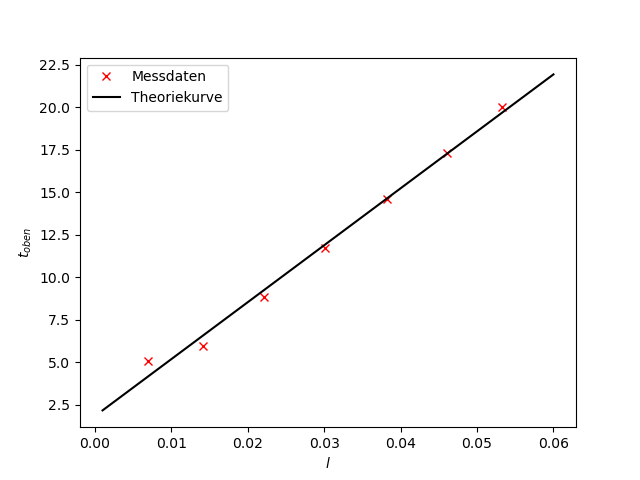
\includegraphics[height=80mm]{bilder/schall.png}
    \caption{Lineare Regression zur Bestimmung der Schallgeschwindigkeit.\label{Abbildung6} }
\end{figure}

\subsection{Untersuchung des Auflösungsvermögen}

\begin{flushleft}
    In dem Acrylblock befinden sich zwei benachbarte Fehlstellen, Lochnummer eins und zwei. 
    Diese werden mit einem A-Scan untersucht. 
    Benutzt wird eine $ 1\,\unit{\mega\hertz} $ Sonde und eine $ 2\,\unit{\mega\hertz} $ Sonde.
    Als Koppelmittel wird Wasser benutzt. 
    Die Grafiken werden exportiert und die Messwerte, wie Laufzeiten und Fehlstelle, werden notiert in Tabelle \ref{Tabelle4}.
\end{flushleft}

\begin{figure}[H]
    \centering
    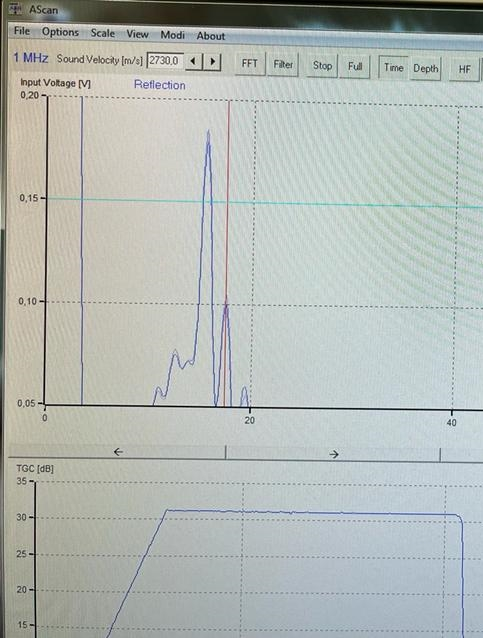
\includegraphics[width=80mm]{bilder/1.jpeg}
    \caption{A-Scan mit einer $ 1\,\unit{\mega\hertz} $ Sonde.\label{Abbildung5} }
\end{figure}

\begin{figure}[H]      
    \centering
    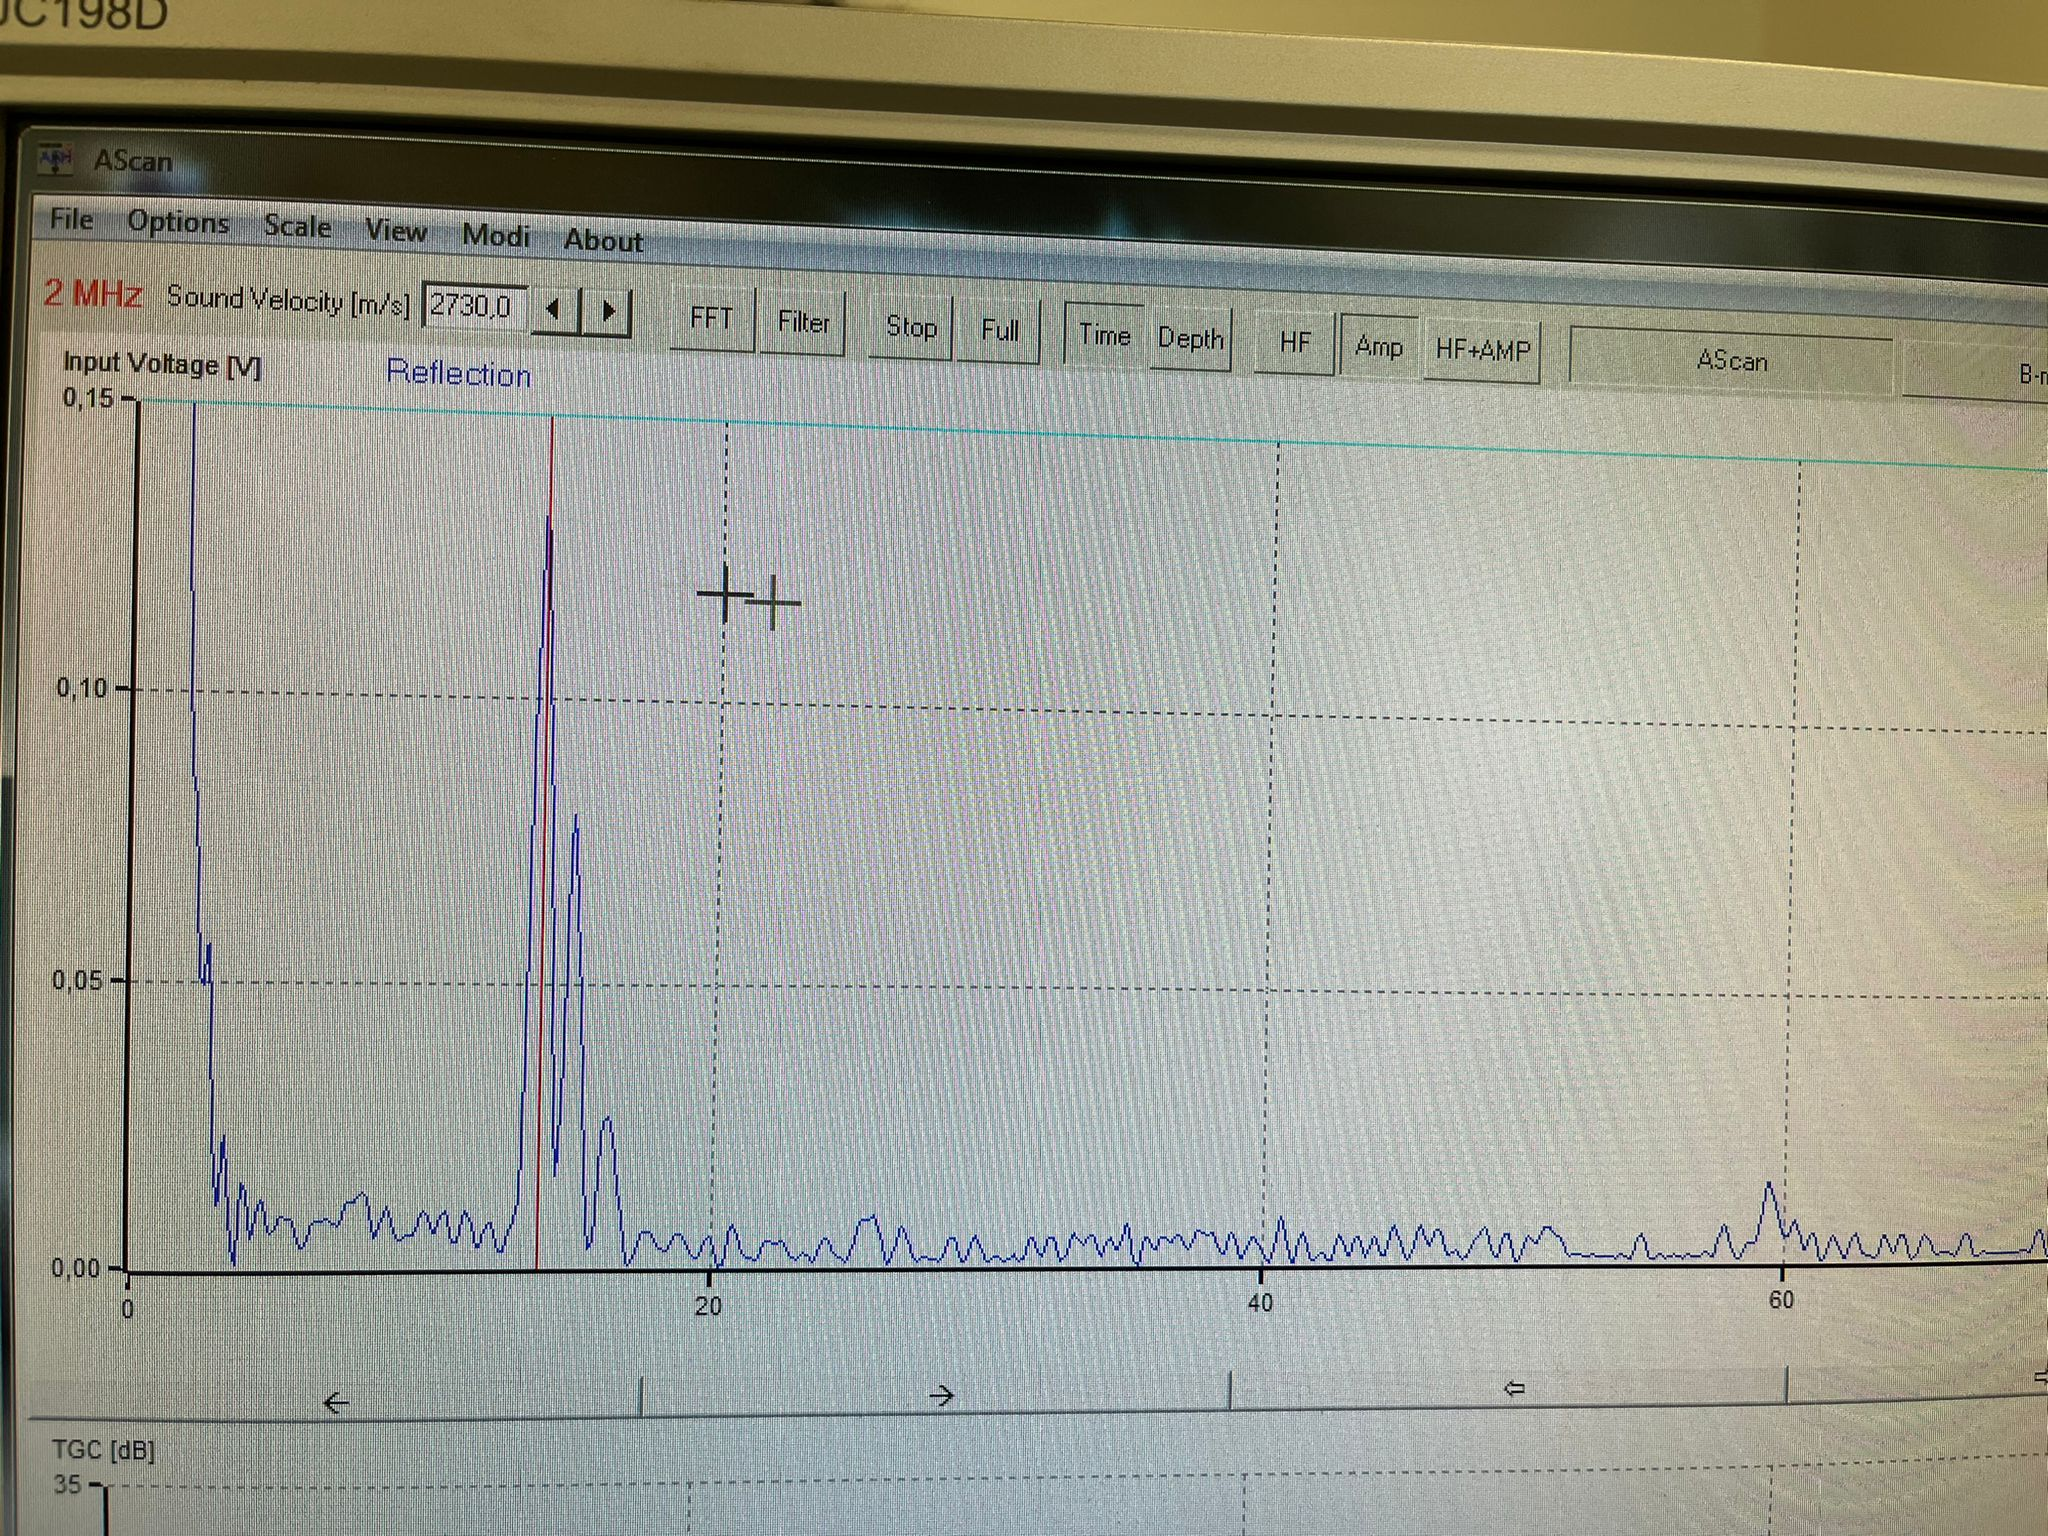
\includegraphics[height=70mm]{bilder/A2 2megahertz.jpeg}
    \caption{A-Scan mit einer $ 2\,\unit{\mega\hertz} $ Sonde.\label{Abbildung2} }
\end{figure}

\begin{table}[H]
    \centering
    \caption{Messungen des zweiten Arbeitsauftrages mit der oberen Kante.} 
    \label{Tabelle4}
    \begin{tabular} {c || c  c || c  c}
        \toprule
        {$ \text{Loch} $} &
        {$ \text{S}_{\text{M}} \mathbin{/} \unit{\milli\second} $} &
        {$ \text{t} \mathbin{/} \unit{\second} $} &
        {$ \text{S}_{\text{M}} \mathbin{/} \unit{\milli\second} $} &
        {$ \text{t} \mathbin{/} \unit{\second} $} \\
        \midrule
        1 & 15,0 & 13,9 & 21,2 & 15,6 \\
        2 & 20,5 & 15,0 & 23,7 & 17,4 \\
        \bottomrule
        {} &
        {$ 2\,\unit{\mega\hertz} $} &
        {} &
        {$ 1\,\unit{\mega\hertz} $} &
        {} \\
    \end{tabular} 
\end{table}

\subsection{Untersuchung der Störstellen mit einem B-Scan}

\begin{flushleft}
    Die Untersuchung erfolgt wie im ersten Teil nur wird ein B-Scan durchgeführt.
    Benutzt wird eine $ 2\,\unit{\mega\hertz} $ Sonde und Wasser als Koppelmittel.
    Die Grafiken werden anschließend exportiert. 
    Die ermittelten Werte aus den Bildern befinden sich in Tabelle \ref{Tabelle5} und wurden mithilfe der Formel (\ref{6}) bestimmt.
\end{flushleft}

\begin{figure}[H]
    \centering
    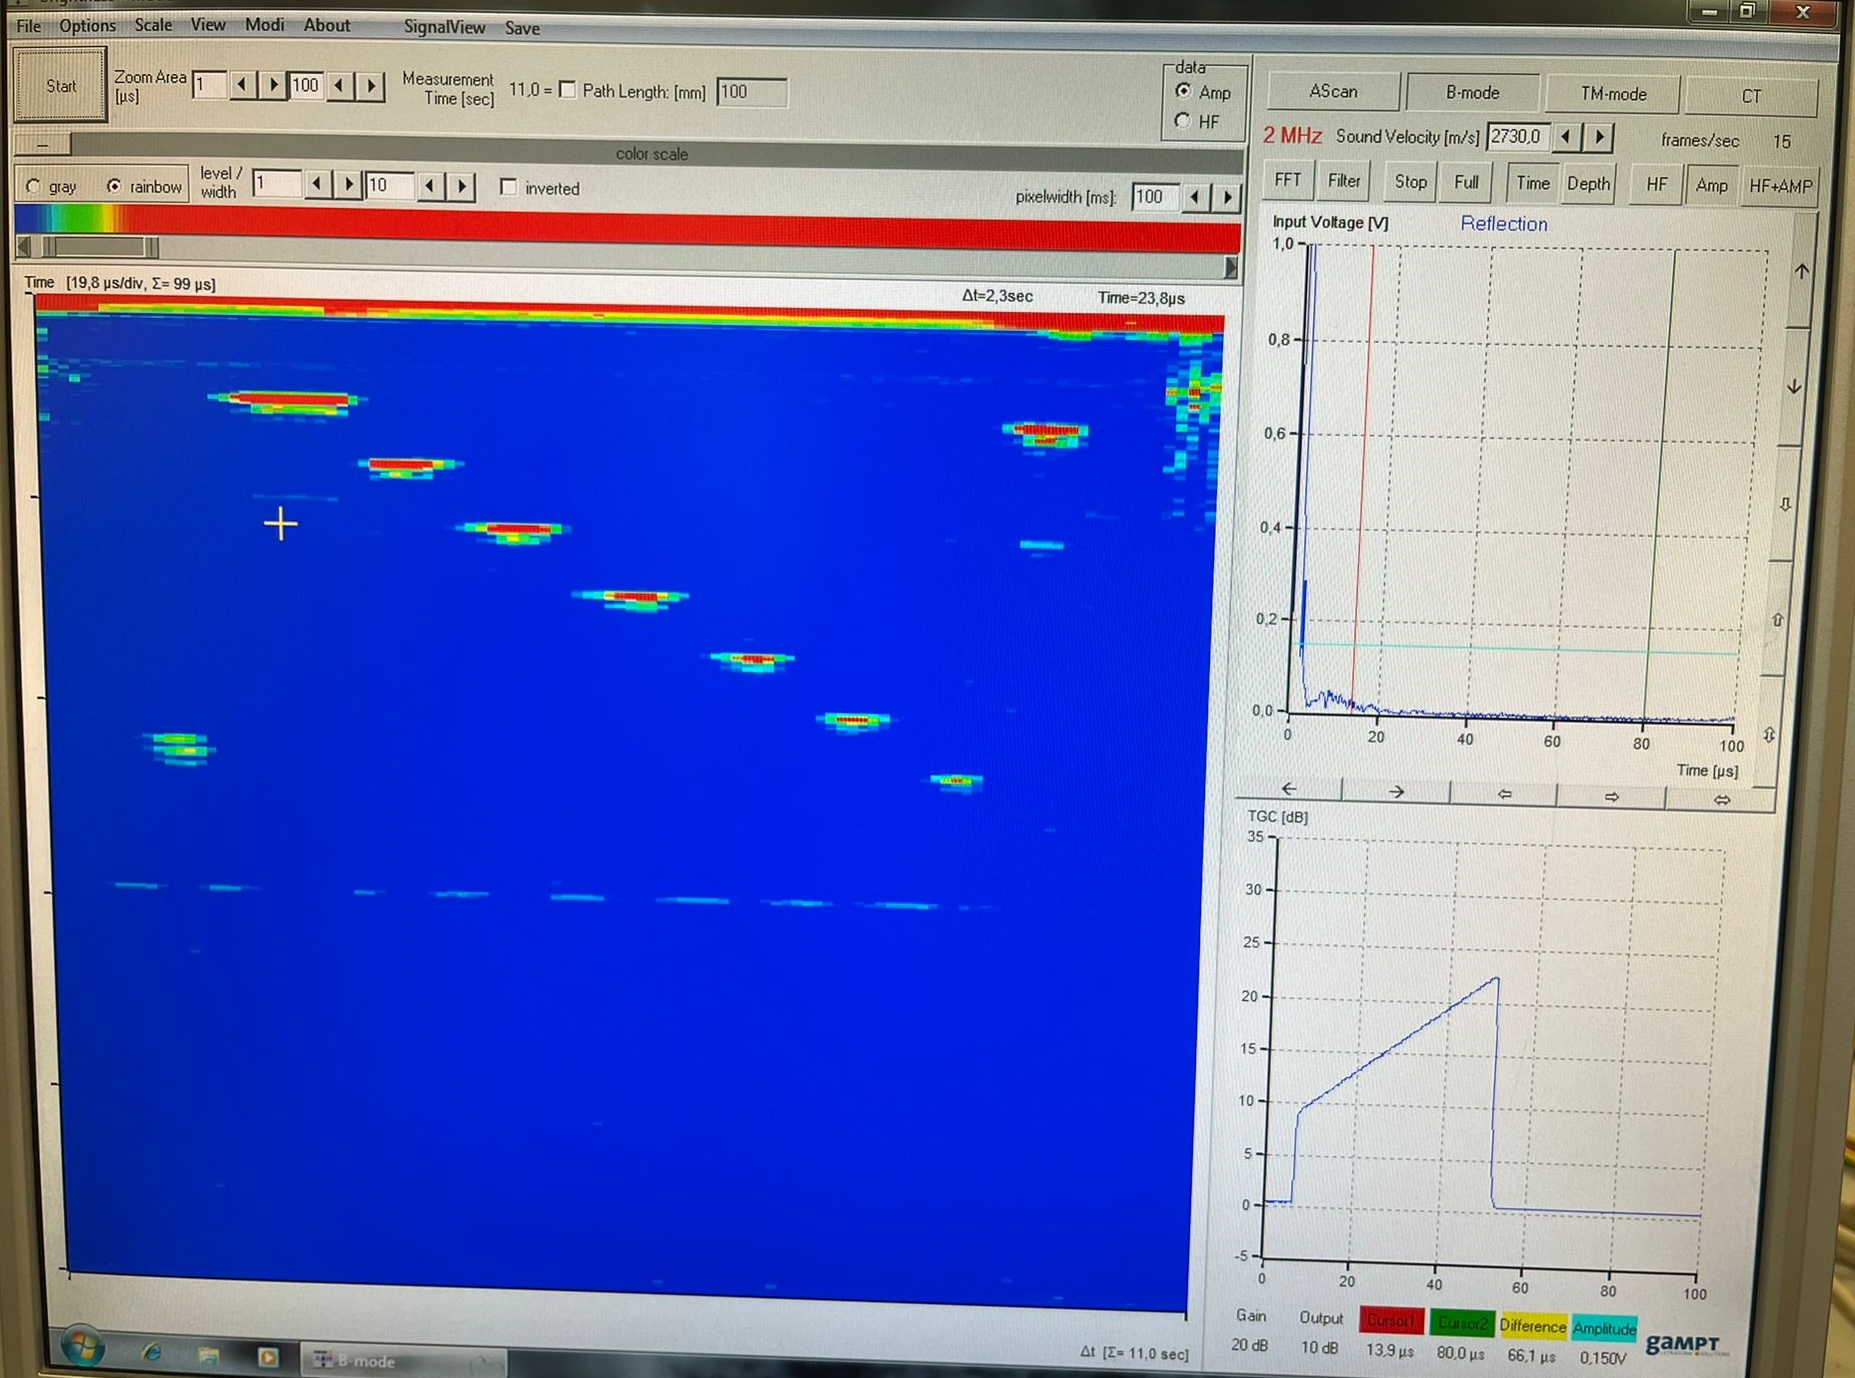
\includegraphics[height=70mm]{bilder/Bscan2.jpeg}
    \caption{B-Scan des Acrylblocks in der ersten Lage.\label{Abbildung3} }
\end{figure}

\begin{figure}[H]
    \centering
    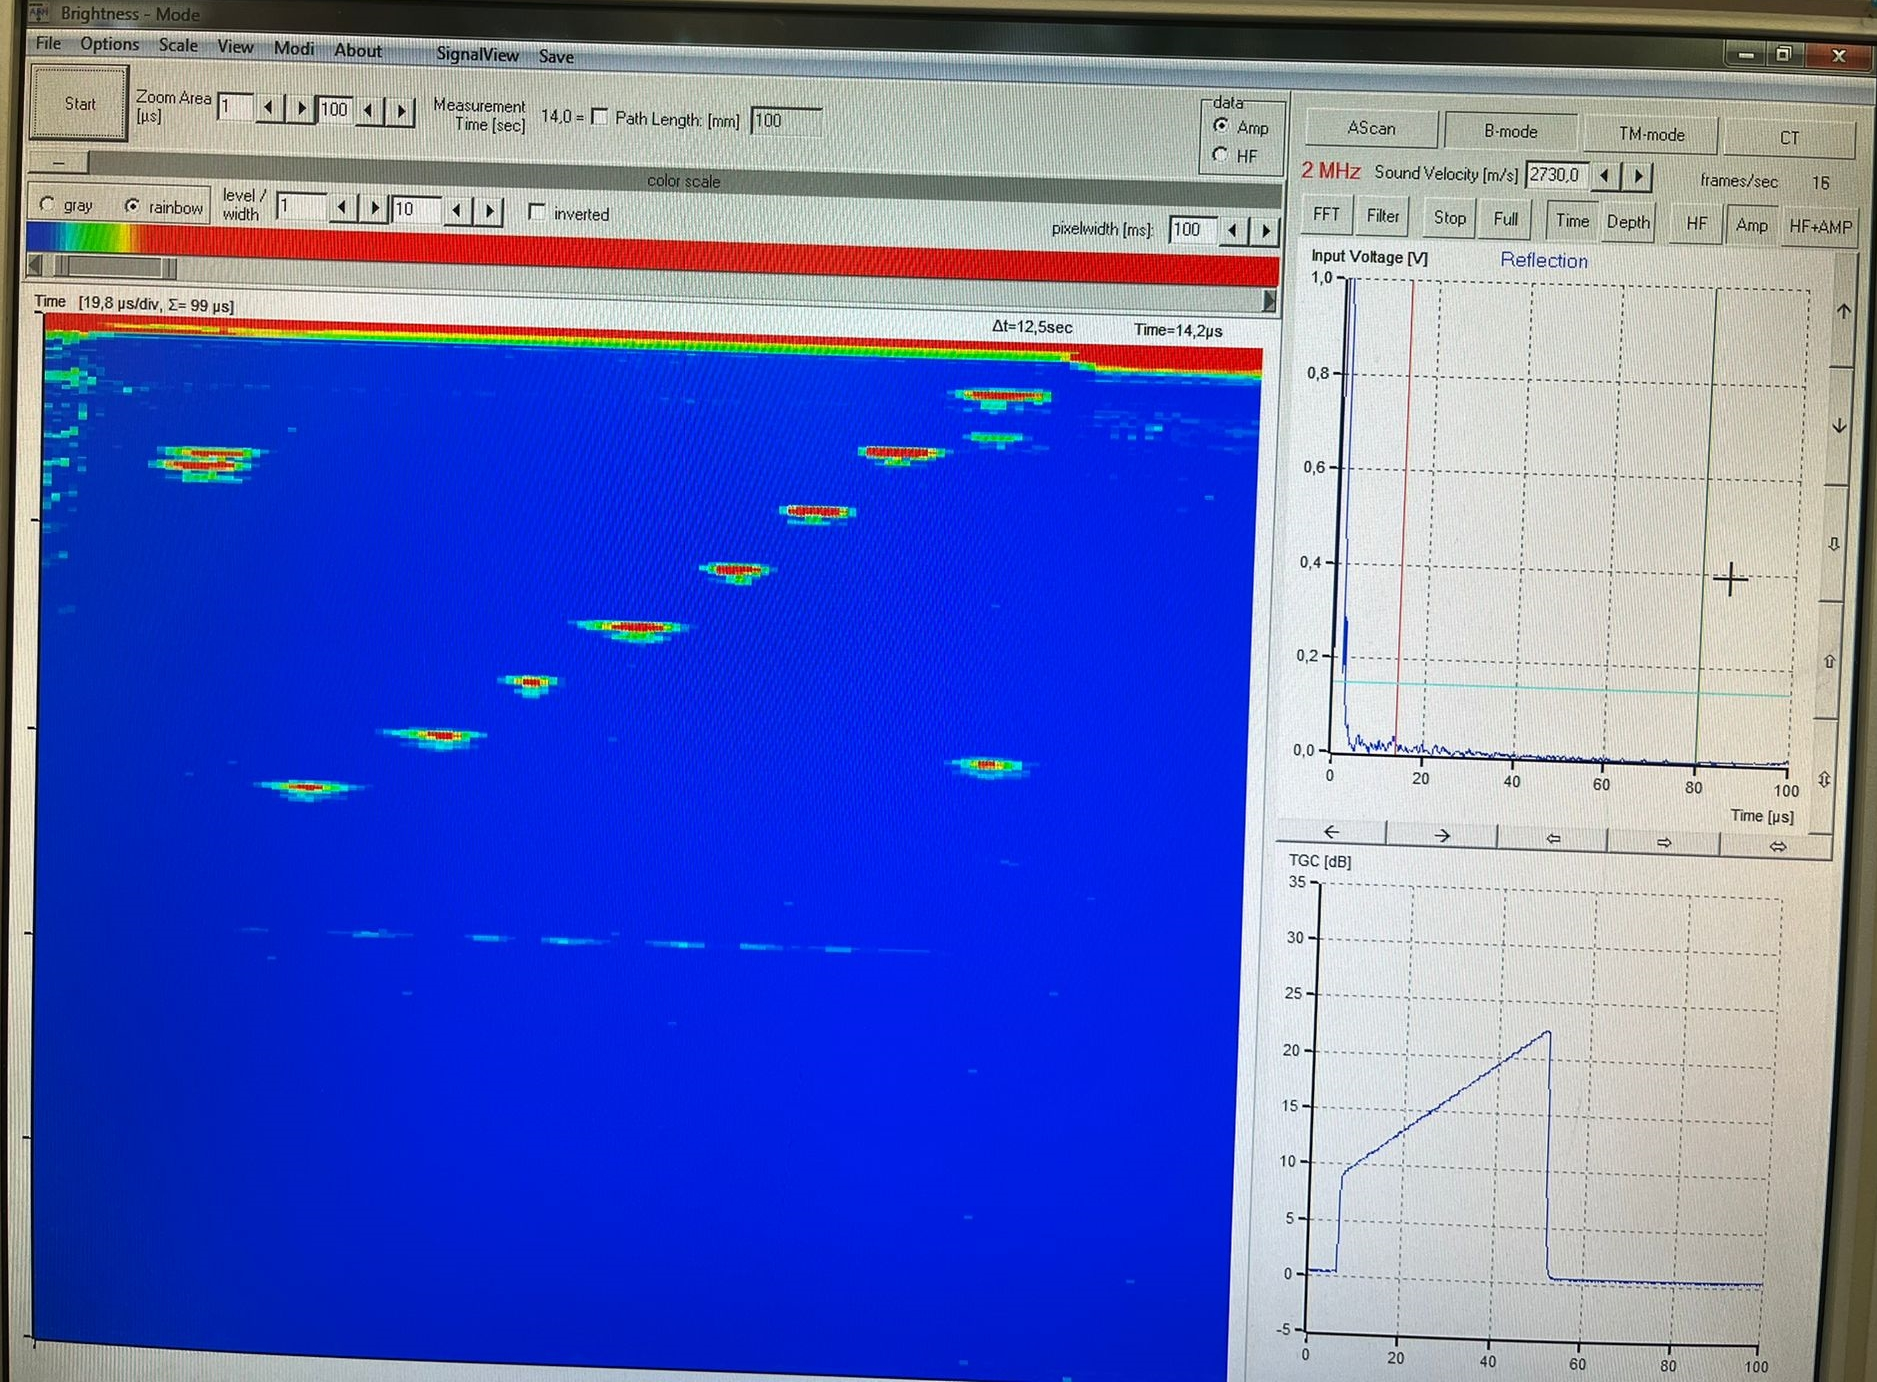
\includegraphics[height=70mm]{bilder/Bscan1.jpeg}
    \caption{B-Scan des Acrylblocks in der zweiter Lage.\label{Abbildung4} }
\end{figure}

\begin{table}[H]
    \centering
    \caption{Messungen des ersten Arbeitsauftrages.} 
    \label{Tabelle5}
    \begin{tabular} {c  c  c  c  c  c}
        \toprule
        {$ \text{Loch} $} &
        {$ \text{t}_{\text{oben}}  \mathbin{/} \unit{\micro\second} $} &
        {$ \text{s}_{\text{oben}}  \mathbin{/} \unit{\micro\second} $} &
        {$ \text{t}_{\text{unten}} \mathbin{/} \unit{\micro\second} $} &
        {$ \text{s}_{\text{unten}} \mathbin{/} \unit{\micro\second} $} \\
        \midrule
        4  & 41,0 & $ 55,96 \pm 0,18 $ & 17,8 & $ 24,29 \pm 0,08 $ \\
        5  & 35,7 & $ 51,46 \pm 0,17 $ & 23,5 & $ 32,07 \pm 0,11 $ \\
        6  & 30,3 & $ 41,35 \pm 0,13 $ & 29,9 & $ 40,81 \pm 0,12 $ \\
        7  & 24,3 & $ 33,16 \pm 0,11 $ & 36,0 & $ 49,14 \pm 0,16 $ \\
        8  & 18,6 & $ 25,38 \pm 0,08 $ & 42,1 & $ 57,46 \pm 0,18 $ \\
        9  & 12,9 & $ 17,60 \pm 0,07 $ & 49,1 & $ 67,02 \pm 0,22 $ \\
        10 & 7,2  & $ 9,82  \pm 0,04 $ & 34,6 & $ 47,29 \pm 0,16 $ \\
        \bottomrule
    \end{tabular} 
\end{table}